\documentclass{article}

\usepackage[final, nonatbib]{nips_2017}
% \usepackage{nips_2017}

\usepackage[utf8]{inputenc} % allow utf-8 input
\usepackage[T1]{fontenc}    % use 8-bit T1 fonts
\usepackage{hyperref}       % hyperlinks
\usepackage{url}            % simple URL typesetting
\usepackage{booktabs}       % professional-quality tables
\usepackage{amsfonts}       % blackboard math symbols
\usepackage{nicefrac}       % compact symbols for 1/2, etc.
\usepackage{microtype}      % microtypography
\usepackage{graphicx}		% images


\graphicspath{{images/}}

\title{MNIST Classification with Deep Convolutional Neural Networks}

\author{
  Aaron G.~Alphonsus \\
  Department of Computer Science \\
  South Dakota School of Mines and Technology \\
  Rapid City, SD, 57701 \\
  \texttt{aaron.alphonsus@mines.sdsmt.edu} \\
}

\begin{document}
% \nipsfinalcopy is no longer used

\maketitle

% Here's an 81 char comment:
%0123456789012345678901234567890123456789012345678901234567890123456789012345678X

% 4-8 sentences
\begin{abstract}
	Deep Neural Networks have regularly achieved state-of-the-art results especially in the field of image classification. AlexNet in 2012, was one such groundbreaking network which achieved a near 50\% reduction in the error rate of the previous state-of-the-art model. In this project, we have implemented some of the core architectural elements of AlexNet using the TensorFlow framework. We picked the MNIST dataset and created a deep convolutional neural network to classify it. With our model, we were able to match some of the best models from the last 10 years and achieve a near state-of-the-art result of 99.2\% test accuracy. Our next steps include implementing batch normalization to improve our model, and utilizing real-time data visualization techniques to better understand the dataset and training process. 
\end{abstract}


% Less than 20% (1.2 pages) Don't exceed 25% (1.5 pages)
\section{Introduction}

The objective of this project was to pick a framework and dataset, and get 
a deep neural network trained and its performance tested. We took a few stabs at 
this with different frameworks and datasets and realized there was a steep 
learning curve to it. As this was our first time doing a machine learning 
project we decided to narrow the scope of the project classifying the 
introductory-level MNIST \cite{mnist} dataset using the popular TensorFlow framework.  

In Dr. McGough's lectures on convolutional networks \cite{convnets}, we were introduced to the history of the convolutional neural network and how they exploded on the scene. It was here that we saw the architectural features of AlexNet and learned how influential it was to the field at the time. The network from the original paper can be seen in figure \ref{fig:alexnet}. Note that the computation is divided into two pipelines showing the authors' use of 2 GPUs in training their network.

\begin{figure}[h]
	\centering
	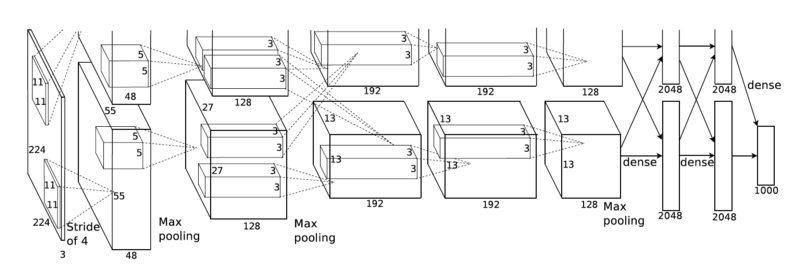
\includegraphics[width=\textwidth]{alexnet.png}
    \caption{AlexNet convolutional neural network architecture}
    \label{fig:alexnet}
\end{figure}

The paper by Alex Krizhevsky proposed using a Deep Convolutional Neural Network for the task of image classification. The dataset that they used was the ImageNet dataset \cite{alexnet}. Looking at the results they obtained, we thought we could use the features of their network and get some good results for a simple image dataset like MNIST. 

We began by implementing a simple single-layer neural network using TensorFlow to get used to the platform \cite{tutorial}. This yielded a modest 92\% accuracy rate on the dataset. This is not great for the MNIST dataset, but creating the network did give us an end-to-end solution and it also got us familiar with the concepts and syntax.  

We then moved on to implementing a deep convolutional network making use of dropout, ReLU neurons, successive convolution and pooling layers, and a densely connected final layer \cite{tutorial-cnn}. These were all features that were also used in AlexNet \cite{alexnet-features}. This model was a lot more successful, achieving an accuracy of 99.2\%. 

After we had the deep network implemented, we tested a few things out like different gradient descent optimizers, editing the network structure, and getting rid of dropout. We also wanted to work on being able to share our model without needing the user to spend time retraining it. Having the smaller model really helped here, as it meant we could test out edits without having to spend a lot of time waiting for the deep network to train. We weren't able to optimize the model further, but we were able to implement saving and restoring of the trained model.

% No specific limit. ~25% of paper 
\section{Methods and Materials}

\subsection{Initial Choices}

In tackling this project we had a few important decisions to make right up front. These were mainly picking a dataset to classify, and picking the framework. With not a lot of background information to make that decision, we probably picked something a little out of reach that we needed to work up to. After a lot of time spent spinning our wheels trying harder datasets, we decided to go simple and pick TensorFlow and MNIST. 

\subsubsection{The Framework}

Choosing a framework when you are a machine learning beginner is a little daunting. There are a lot to choose from and a lot of people batting for each one. We decided to go with TensorFlow because of its popularity and flexibility. We guessed that its popularity would mean better documentation, tutorials, and help along the way. Also, we figured that it is the framework that we will most likely need to use again in our career, be it academia or industry. With that said, there are probably easier ones to get started with, especially those built on TensorFlow that advertise rapid prototyping such as Keras. 

\subsubsection{The Dataset}

The MNIST dataset is popularly referred to as a "sanity check" dataset. This is because it is a relatively small dataset with not many categories. You can test out your new architecture quickly with it before turning it loose on your bigger datasets. This also means that it is a popular dataset among machine learning beginners. Having been unsuccessful getting a more complex dataset working, we decided to target MNIST in our project.

MNIST is a computer vision dataset. Each example is a gray-scale 28x28 pixel image and contains a handwritten digit from 0 to 9. Each digit has been centered in the 28x28 image. An example of the handwritten digits contained in the MNIST dataset can be seen in figure \ref{fig:mnist}. The dataset has a training set of 60,000 examples and a test set of 10,000 examples. Since each image is a 0-9 digit, it is a 10 category dataset.

\begin{figure}[h]
	\centering
    \fbox{
\includegraphics[width=0.15\textwidth]{mnist5.png}}\quad
    \fbox{
\includegraphics[width=0.15\textwidth]{mnist0.png}}\quad
    \fbox{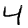
\includegraphics[width=0.15\textwidth]{mnist4.png}}\quad
    \fbox{
\includegraphics[width=0.15\textwidth]{mnist1.png}}
    \caption{Examples of the handwritten digits in MNIST}
    \label{fig:mnist}
\end{figure}

\subsection{Network Architecture}

In our first attempt we built a softmax regression model with a single linear layer. Assuming our input image vector to be $x$, the weight matrix to be $W$, and the bias vector to be $b$, our regression equation is as follows:
\[y = x.W + b\]
where $y$ is the model's prediction and the '$x.W$' operation is a matrix multiplication. The architecture for this model can be seen in figure \ref{fig:mnist-single-architecture}

\begin{figure}[h]
	\centering
	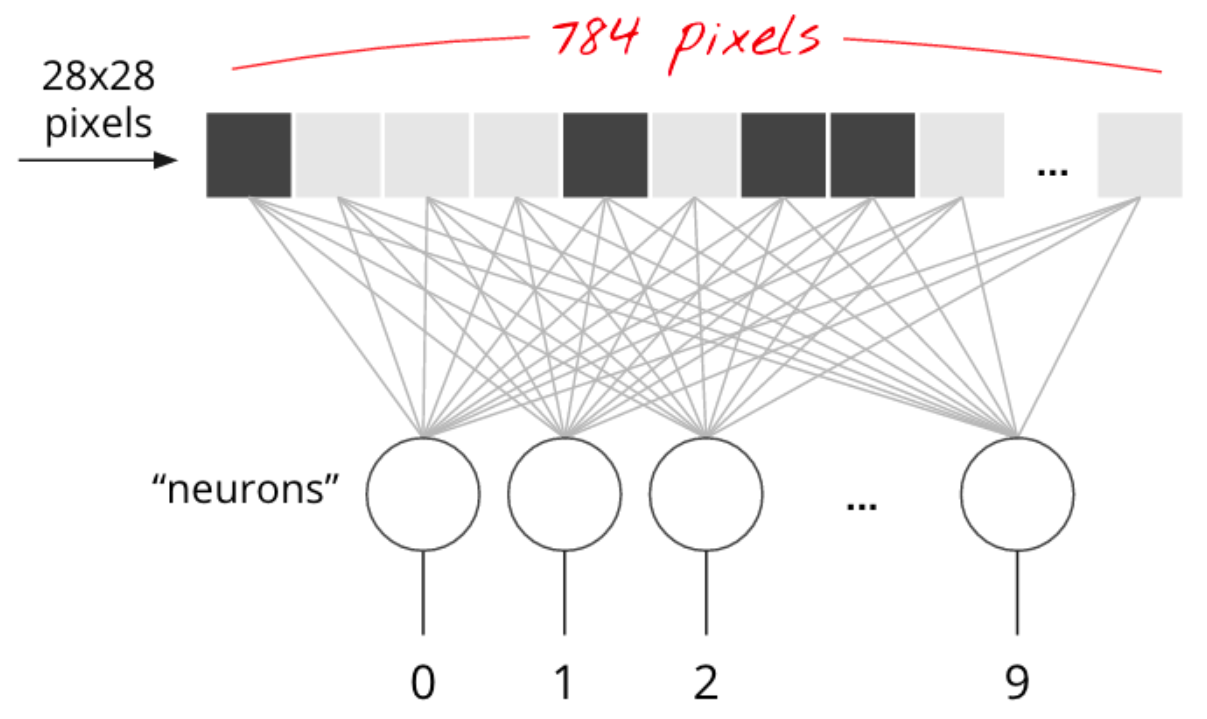
\includegraphics[width=0.7\textwidth]{mnist-single-architecture.png}
    \caption{Network architecture of the single-layer neural net}
    \label{fig:mnist-single-architecture}
\end{figure}

As mentioned earlier, our network architecture uses a lot of elements from AlexNet, as do a lot of neural networks that have come after it. AlexNet contains 60 million parameters and 650,000 neurons. It has 5 convolutional layers (3 of which are followed by max-pooling), 3 fully connected layers, and a final 1000-way softmax. Looking at the features from AlexNet, we implemented a neural network with the following features in its network architecture:
\begin{itemize}
	\item ReLU for the activation functions.
    \item 2 convolution layers, each followed by max pooling.
    \item A final densely-connected layer.
    \item A single linear readout layer 
\end{itemize}
The architecture for this network can be seen in figure \ref{fig:mnist-deepcnn-architecture}

\begin{figure}[h]
	\centering
	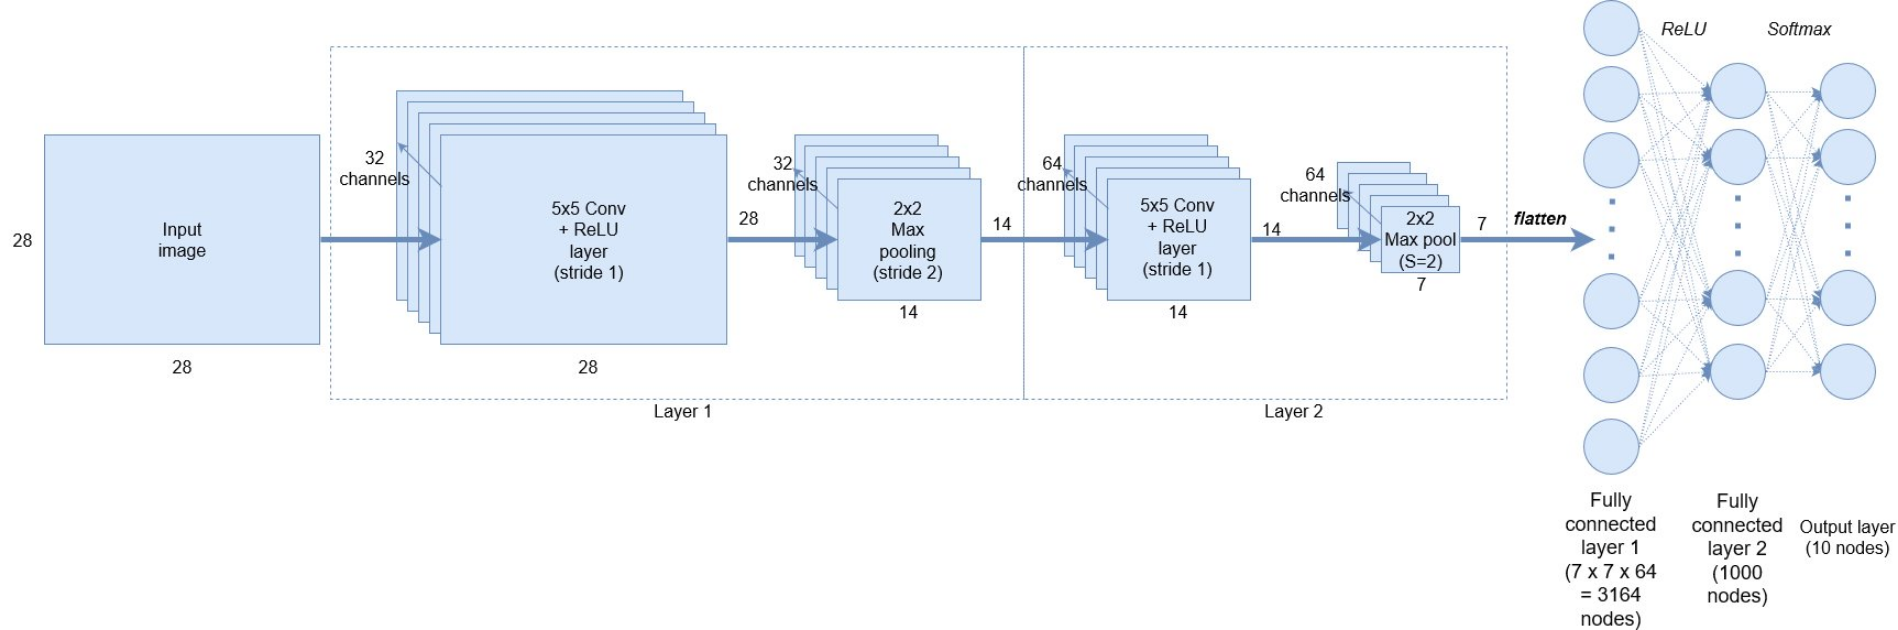
\includegraphics[width=\textwidth]{mnist-deepcnn-architecture.png}
    \caption{Network architecture of the deep convolutional neural net}
    \label{fig:mnist-deepcnn-architecture}
\end{figure}

Building the model in TensorFlow was not very involved once we got the hang of the syntax. It was the theory behind the model that took the most time to understand. This was helped along towards the end of our project with a few lectures in class covering theory and some code for convolutional neural nets. 

Our input variable contains a 2D tensor of floating point numbers where the first dimension is the variable batch size and the second is the linearized 28x28 pixel image. The target output class variable is a 2D tensor where each row is a one-hot 10-dimensional vector and it indicates the digit class (0-9) that the MNIST image belongs to.

% \subsection{The Method}

% Our script begins by loading the MNIST dataset into a lightweight class that stores the training, validation, and testing sets as NumPy arrays. Our input variable contains a vectorized 28x28 pixel MNIST image. The target output class variable is a 2D tensor where each row is a one-hot 10-dimensional vector and it indicates the digit class (0-9) that the MNIST image belongs to.

%\subsection{Other Elements of the Model}

\subsection{Optimizations}

After we implemented the network using TensorFlow, we turned our attention to the task of hyperparameter tuning and optimization of the model. TensorFlow provides a number of built-in options to tweak your model and this is what we experimented with. We also read up on techniques used to improve a deep convolutional neural network such as dropout regularization which is used to stop neural networks from overfitting \cite{srivastava2014dropout}.

The model we emulated included dropout but it came with a footnote explaining that the technique wasn't as important as it is to large neural networks. The network we trained isn't quite on the scale of some of the models out there where overfitting is a significant problem. We experimented with leaving out the dropout regularization method but as it turns out, we do have some over-fitting even with this model. Keeping dropout in was essential to maintaining those valuable tenths decimal places in our model's accuracy rating.

The next thing we tried was the different gradient descent optimizers - something that TensorFlow provides a lot of built-in options for. Our model made use of the Adam optimizer, which we had heard of in class, and one that Ian Goodfellow, the author of our textbook recommends \cite{goodfellow2016nips}. We tried a couple of different optimizers including Adagrad and the default GradientDescentOptimizer along with varying the learning rate initialization value for all the optimizers. Seeing marginal changes in accuracy, we decided to move on to something else.

\subsection{Saving and Restoring}

After taking a crack at optimizing our model with not too much to show for it, we decided to look at being able to save our trained model. We figured it would be a useful feature to be able to demonstrate the classification without the wait time of having to train the model. This was also motivated by the guest lecture from Dr. Hoover who demonstrated an MNIST classifier that had the weights of the model saved so that it could be restored quickly and used on the dataset.

It turned out TensorFlow had a method that could do this, however it was not quite the same as saving and loading the individual variables used. While this meant the code to achieve the feature was simple in the end, figuring out exactly what needed to be done and testing it took some time. Having the smaller single-layer network was crucial here as we were able to quickly get the results on what we tried because of the low training time.

% subsection framework?
% Diagrams of the training

% Up to 50% of the paper (3 pages)
\section{Results}

Our first attempt at the MNIST classification problem was with the single-layer neural net with the softmax activation function. Being quite small, this model trains relatively quickly and achieves a test accuracy of around 92\%. In figure \ref{fig:mnist-single} you can see the accuracy being plotted as the model is being trained.

\begin{figure}[h]
	\centering
	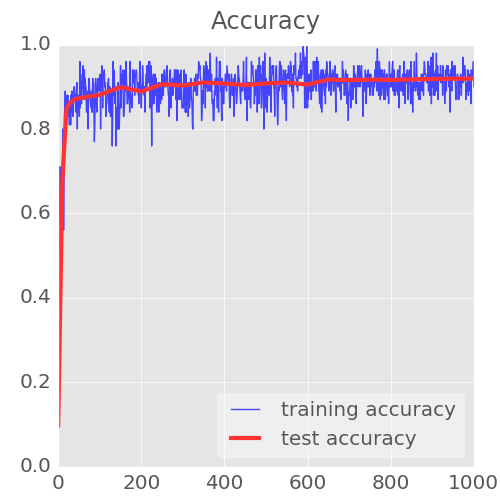
\includegraphics[width=0.5\textwidth]{mnist-single.png}
    \caption{Accuracy plot during the training of the single-layer neural net}
    \label{fig:mnist-single}
\end{figure}

In our next attempt, we implemented a deep convolutional neural network using features from some of the best models that have classified the dataset. This model takes considerably longer to train when compared to our first model and achieves an accuracy of 99.2\%. Figure \ref{fig:mnist-deepcnn} displays the accuracy plotted as the model is being trained.

\begin{figure}[h]
	\centering
	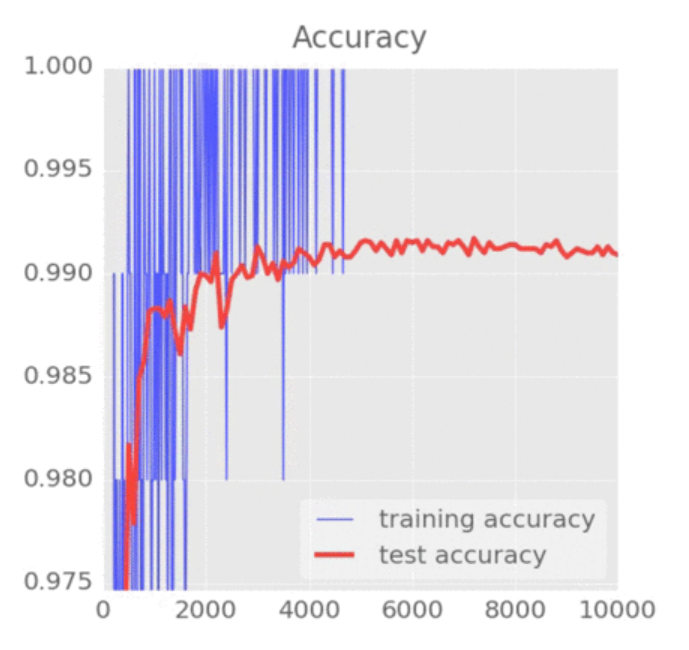
\includegraphics[width=0.55\textwidth]{mnist-deepcnn.png}
    \caption{Accuracy plot during the training of the deep convolutional neural net}
    \label{fig:mnist-deepcnn}
\end{figure}

Using our deep convolutional network, we were able to achieve respectable results on the MNIST dataset. Comparing it to past results, as recorded by the creator of the dataset Yann LeCun, our accuracy of 99.2\% puts us amongst the best models, albeit somewhere near the lower end of the pack. As expected, our single-layer model's accuracy of 92\% isn't good enough for this dataset when compared to the state-of-the-art models. It does hold its own against other models of its type, but surely that's only because nobody is actually going to publish a model with that kind of accuracy in current times. Table \ref{table:results} gives a listing of a sampling of the top models of each type for the classification of MNIST.

\begin{table}[h]
	\caption{Sampling of MNIST results for similar models}
	\centering
	\begin{tabular}{llll}
        \toprule
        Classifier & Preprocessing & Accuracy (\%) & Year \\
        \midrule
        \multicolumn{3}{c}{\textbf{Linear Classifiers}} \\
		\midrule
        Linear classifier (1-layer NN) \cite{lecun-98} & None & 88.0 & 1998 \\
        Linear classifier (1-layer NN) \cite{lecun-98} & Deskewing & 91.6 & 1998 \\
        Pairwise linear classifier \cite{lecun-98} & Deskewing & 92.4 & 1998 \\
        \midrule
        \multicolumn{3}{c}{\textbf{Convolutional Nets}} \\
		\midrule
        Convolutional net LeNet-1 \cite{lecun-98} & Subsampling to 16x16 & 98.3 & 1998 \\
        Large conv. net, random features \cite{ranzato-cvpr-07} & None & 99.11 & 2007 \\
        Boosted LeNet-4 \cite{lecun-98} & None & 99.3 & 1998 \\
        Large conv. net, unsup features  \cite{ranzato-cvpr-07} & None & 99.38 & 2007 \\
        Large conv. net, unsup pretraining \cite{jarrett-iccv-09} & None & 99.47 & 2009 \\
        Committee of 35 conv. net \cite{DBLP:journals/corr/abs-1202-2745} & Width normalization & 99.77 & 2012 \\
		\bottomrule
	\end{tabular}
    \label{table:results}
\end{table}

% Conclusions and future work
% No more than 20%. Can be less than 5%
\section{Discussion}

Working on this project served as a good introduction both in understanding the architecture of a deep convolutional network, and getting familiar with the TensorFlow framework. We followed along with an introductory TensorFlow tutorial to get introduced to these new concepts as well as the low-level APIs of the framework.

The next step in continuing to develop our understanding of deep learning would 
be to try to incorporate some real-time visualization tools. Some exciting 
tools we have seen being used to visualize data during the training process are TensorBoard and matplotlib. Figure \ref{fig:matplotlib} shows some of the useful plots matplotlib offers while training on the MNIST dataset.

\begin{figure}[h]
	\centering
	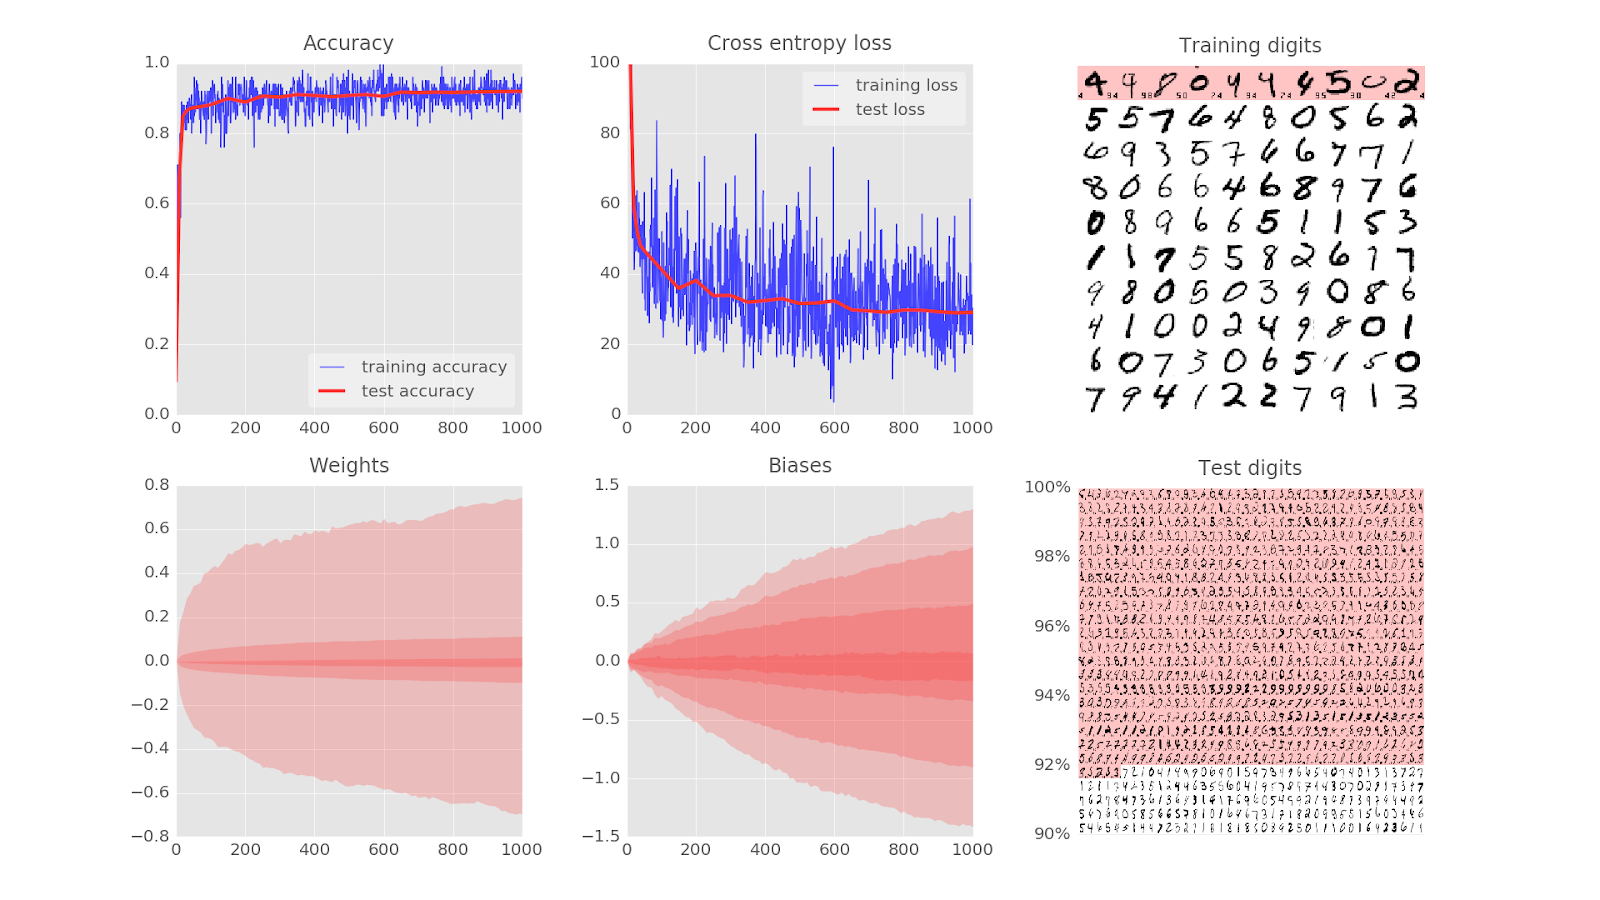
\includegraphics[width=\textwidth]{matplotlib.png}
    \caption{Some useful data visualization tools offered by matplotlib}
    \label{fig:matplotlib}
\end{figure}

In working on this project we used TensorFlow to train a deep network and were able to get respectable results on a popular dataset. We looked at the influential AlexNet architecture and implemented several features of its network architecture including dropout, ReLU neurons, successive convolution and pooling layers, and a densely connected layer at the end. 

For future work on improving results with this model, we would like to look at some commonly-used data augmentation techniques such as random rotation, shear, and shift. This was a technique used by Krizhevsky as a method of increasing the robustness of their model. We would also like to implement batch normalization which is a technique the best MNIST classifier uses. 

\bibliographystyle{IEEEtran}
\bibliography{sources}

\end{document}